\documentclass[11pt]{article}

\usepackage[czech]{babel}
\usepackage[utf8]{inputenc}

\usepackage{graphicx}
\usepackage{blindtext}
\usepackage{hyperref}
\usepackage{amsmath}
\usepackage{multicol}
\usepackage{abstract}
\usepackage{setspace}
\usepackage{ulem} % podtržení nadpisů
\usepackage{wrapfig} % obtékání obrázků 
\usepackage{lastpage}
\usepackage{fancyhdr}
\usepackage{enumitem}

\pagestyle{myheadings}
\pagestyle{fancy}
\usepackage{wrapfig}
\setlength{\headwidth}{16cm}
\fancyhead[L]{ČVA Apollo 373}
\fancyhead[C]{Pracovní list č.1}
\fancyhead[R]{Gymnázium Českolipská}

\setlength{\voffset}{-1.5cm}
\setlength{\textheight}{22.0cm} 
\setlength{\hoffset}{-1.5cm} 
\setlength{\textwidth}{16cm}

\renewcommand{\footrulewidth}{1pt}
\lfoot{\href   {https://www.instagram.com/ceskolipska_vesmirna_agentura/}{IG: @ceskolipska\_vesmirna\_agentura}}


\rfoot{\href{https://www.facebook.com/ceskolipska.vesmirna.agentura/}{FB:  ceskolipska.vesmirna.agentura}}

\usepackage{titlesec}
\titleformat{\subsection}
  {\normalfont\large}{\thesubsection.}{1em}{\uline}

\makeatletter
\setlength{\@fptop}{0pt}
\makeatother


\title{\vspace{-2cm}{\Huge \textbf{Atmosféra}}}
\author{Pracovní list č. 1}
\date{Českolipská vesmírná agentura}
%%%%%%%%%%%%%%%%%%%%%%%%%%%%%%%%%%%%%%%%%%%%%%%%%%%%%%%%%%%%%%%%%%%%%%%%%%%%%%%%%%%%%%%%%%%%%%%%%%%%%%%%%%
\begin{document}
\pagenumbering{gobble}

\maketitle

\begin{center}
\begin{large}

\textbf{Atmosféra je plynný obal Země a lze ji rozdělit do 5 vrstev - 
\newline troposféra, stratosféra, mezosféra, termosféra a exosféra}

\end{large}
\end{center}
%%%%%%%%%%%%%%%%%%%%%%%%%%%%%%%%%%%%%%%%%%%%%%%%%%%%%%%%%%%%%%%%%%%%%%%%%%%%%%%%%%%%%%%%%%%%%%%%%%%%%%%%%

\section{Vrstvy}
%
\subsection*{Troposféra}
%
\begin{wrapfigure}[8]{R}{0.4\textwidth}
 \centering
 \vspace{-2em}
 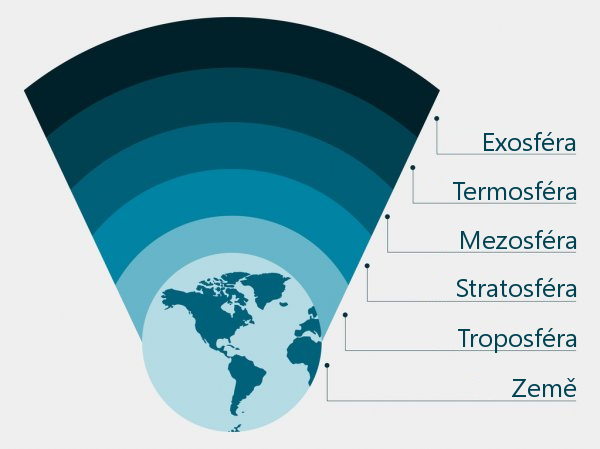
\includegraphics[width=\linewidth]{resources/unknown.png}
\end{wrapfigure}
\paragraph{}
Vrstva nejblíže Zemi. Sahá v průměru do 15 km nad zemský povrch. Jedná se o tři čtvrtiny hmotnosti celé atmosféry mj. proto, že se zde nachází téměř všechna atmosférická voda. V této vrstvě se nejčastěji vyskytují přírodní jevy jako tvorba oblaků, blesků a deště.

%
\subsection*{Stratosféra}
\paragraph{}
Nejnižší část sahá k 10 km a nejvyšší část až do 50 km. Největší zvláštností pro stratosféru je výskyt ozonu $\textrm{O}_3$, vzácné molekuly kyslíku zachytávající UV záření. Velice zvláštními a úžasnými úkazy, které se vyskytují v této vrstvě, jsou tzv. gigantické výtrysky - sloupy plazmy sahající až několik desítek kilometrů.
%
\subsection*{Mezosféra}
\paragraph{} Nejnižší část sahá k $50$ km a nejvyšší část až do $85$ km. Většina meteoritů se vypaří v této vrstvě, kde zanechávají částice železa a dalších kovů. Zvláštními úkazy v této vrstvě jsou tzv. skřítci - načervenalé výboje plazmy.
%
\subsection*{Termosféra}
\par Nejnižší část sahá k 85 km a nejvyšší část až do 1000 km. Díky proměnlivé aktivitě Slunce se tato část splaskává, nafukuje a vyšší hranice se může snížit až k 500 km. Na rozdíl od nižších vrstev se vzduch díky vysoké radiaci ze Slunce skládá z atomů, nikoliv molekul. V této vrstvě se taktéž vyskytuje polární záře, která je způsobena absorpcí fotonů atomy.
%
\subsection*{Exosféra}
\paragraph{} Většinou se horní limit exosféry uvádí na cca. 190 000 km, jelikož zde fotony působí na atomy větší silou než gravitační pole Země. Vzduch v exosféře je tak řídký, že se atomy nesráží. Díky tomu se mohou pohybovat po svých balistických křivkách. Existuje však malá pravděpodobnost, že atom získá dostatek energie a odletí do volného vesmíru.
%
%%%%%%%%%%%%%%%%%%%%%%%%%%%%%%%%%%%%%%%%%%%%%%%%%%%%%%%%%%%%%%%%%%%%%%%%%%%%%%%%%%%%%%%%%%%%%%%%%%%%%%%%%%
\newpage
%
\section{Složení}
%
\begin{wrapfigure}[13]{R}{0.4\textwidth}
 \centering
 \vspace{-2em}
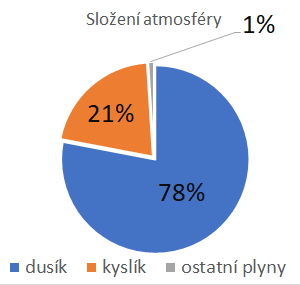
\includegraphics[width=\linewidth]{resources/graf2}
\end{wrapfigure}
%
\paragraph{}
Obecně lze atmosféru Země rozdělit podle složení na čistý vzduch, vodu a aerosoly. Vzduch se skládá z 78 \% dusíku, 21 \% kyslíku a vzácných plynů - argon - popřípadě stopových plynů jako $\textrm{CO}_2$. Celkové zastoupení vody v atmosféře je 4 \% a velká většina se vyskytuje do 10 km, kde ji nalezneme ve všech třech skupenstvích - vodní pára v podobě oblačnosti, kapalná voda ve formě deště a vlhkosti a také krystalky ledu v podobě sněhu. Aerosoly se v atmosféře díky své hustotě vyskytují převážně v té nejnižší vrstvě. Spadá mezi ně hlavně prach a písek ze země, kouř z komínů ale také sůl z moře, pyl z rostlin a kapky chemikálií.
%
%%%%%%%%%%%%%%%%%%%%%%%%%%%%%%%%%%%%%%%%%%%%%%%%%%%%%%%%%%%%%%%%%%%%%%%%%%%%%%%%%%%%%%%%%%%%%%%%%%%%%%%%%%
\section{Historie meteorologie}
%
\begin{wrapfigure}[12]{R}{0.3\textwidth}
 \centering
 \vspace{-2em}
 \href{https://www.youtube.com/watch?v=dQw4w9WgXcQ}{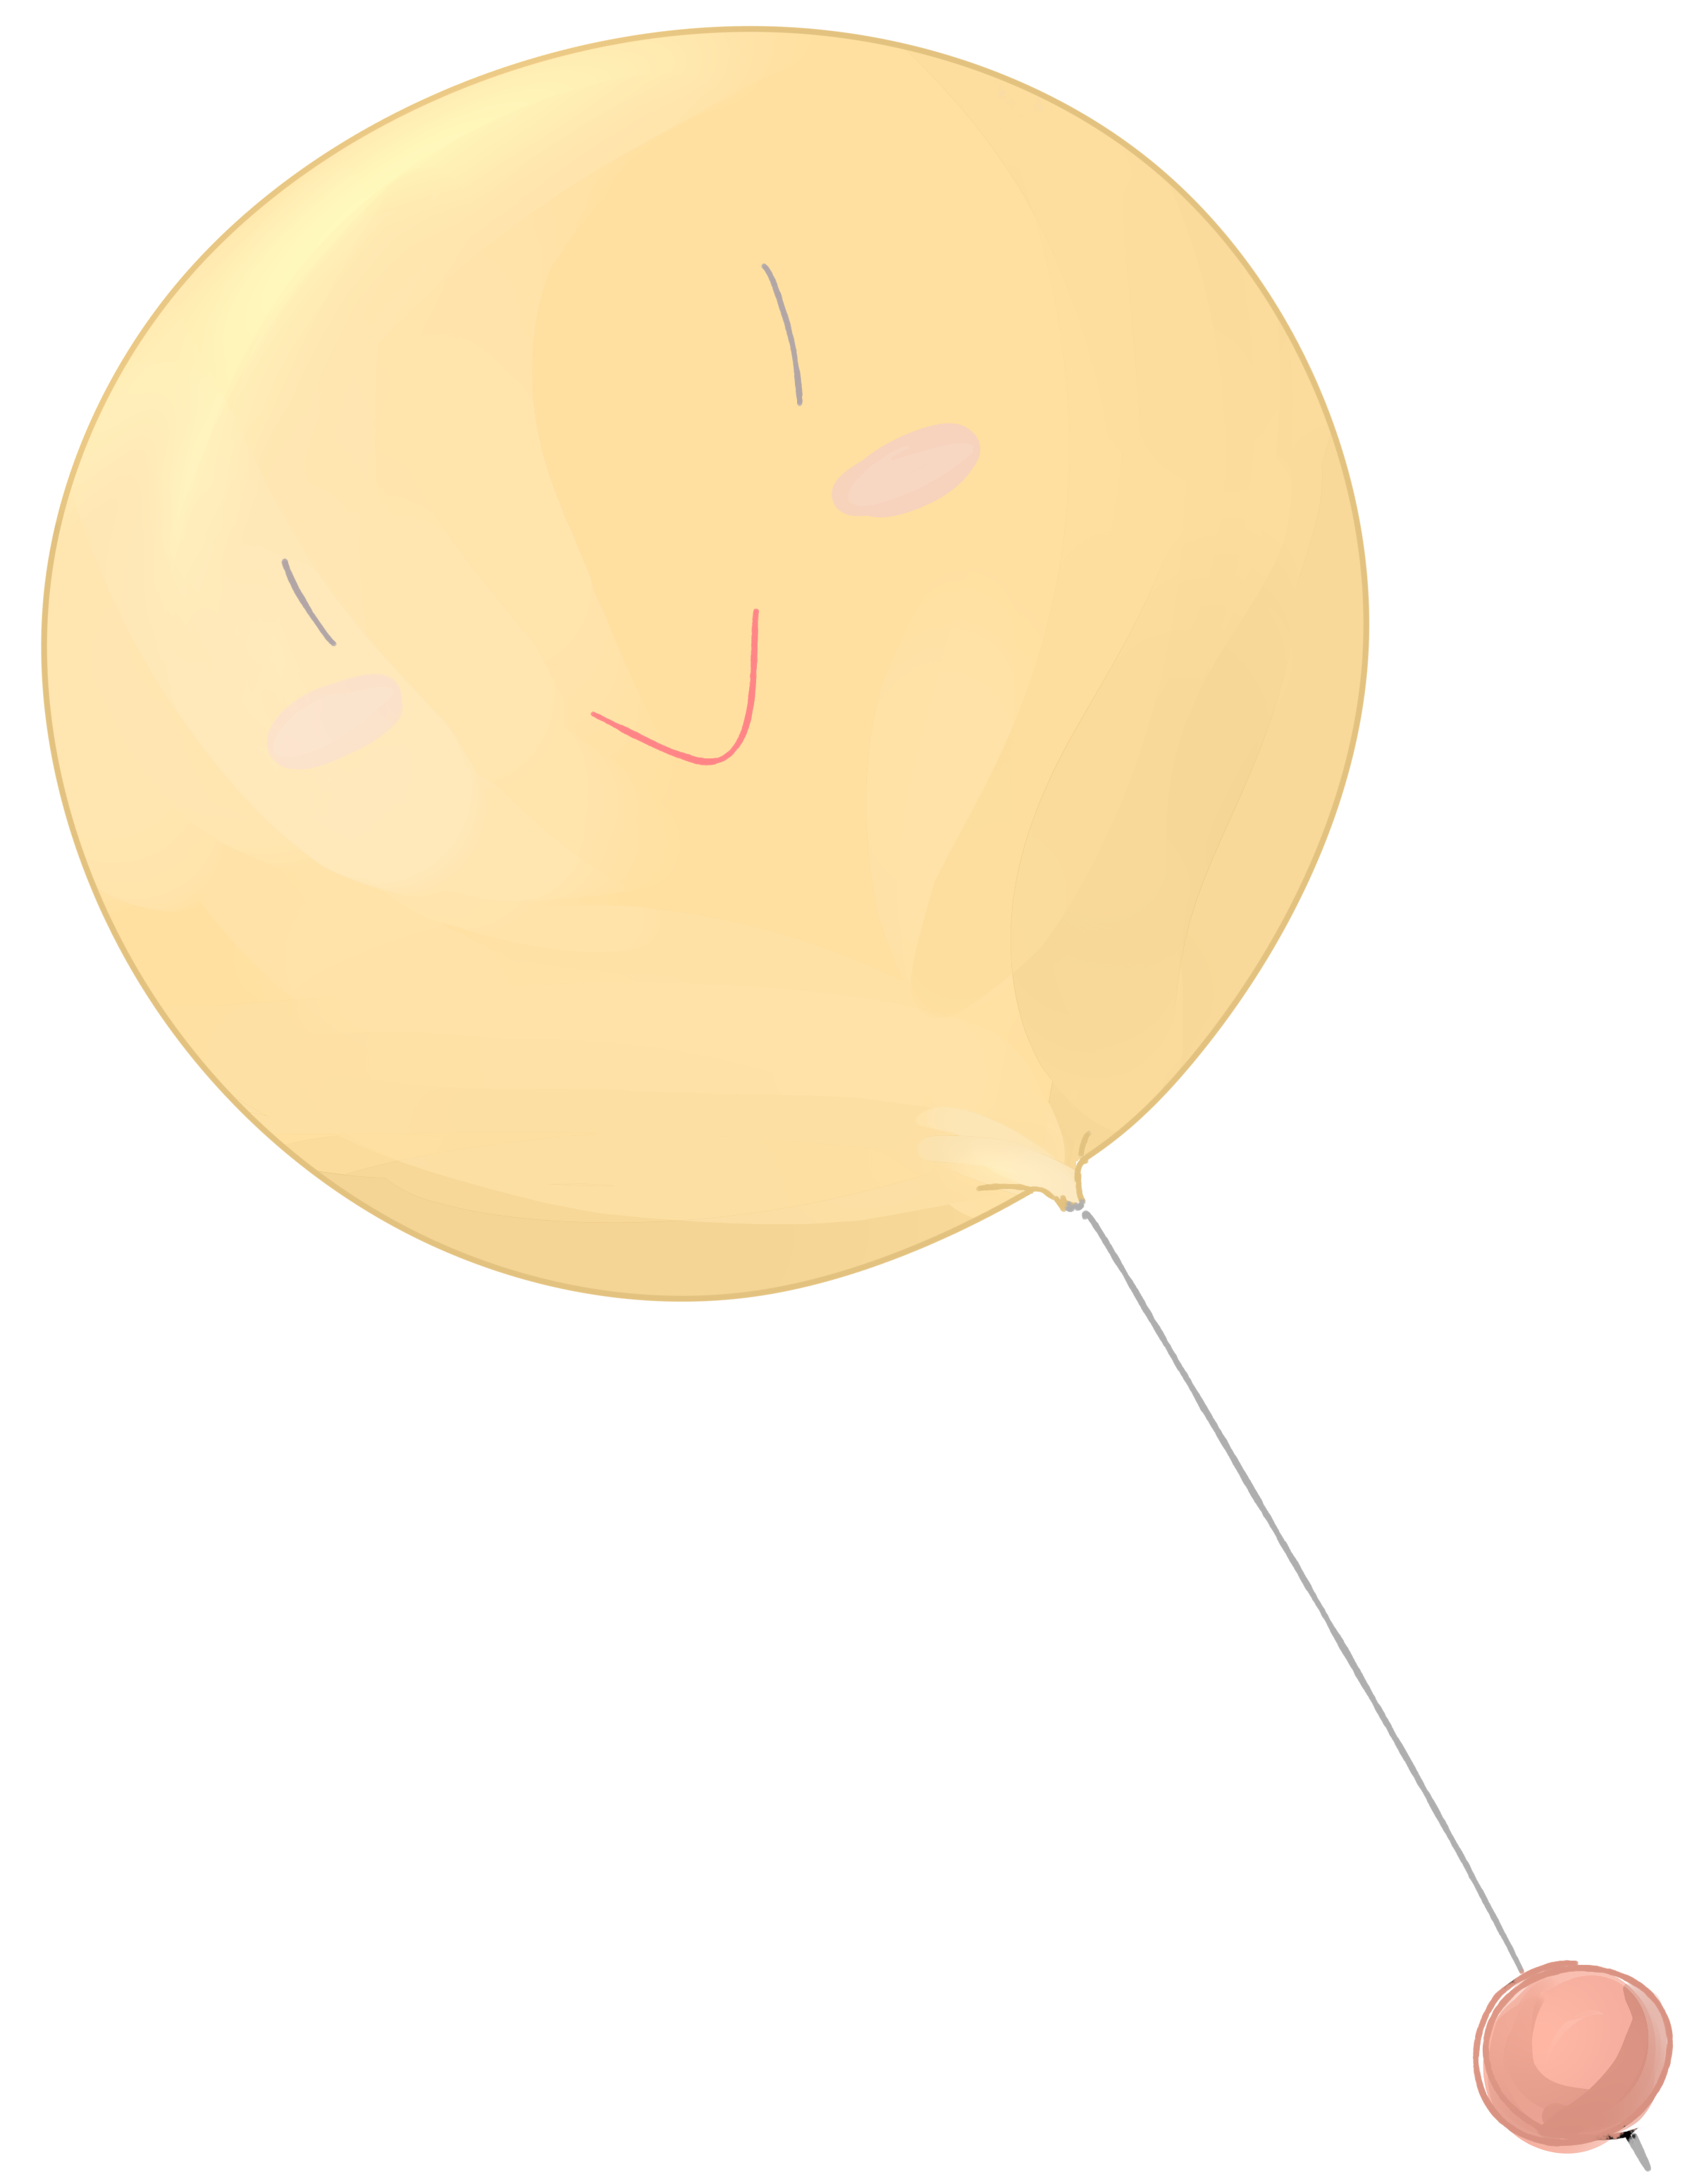
\includegraphics[scale=0.38]{resources/balon.png}}
\end{wrapfigure}

%
\par
%
\paragraph{}
Meteorologie v prastarých časech byla pouze o předpovídání počasí na základě okem viditelných atmosférických jevů, cyklů a chování zvířat. Nejednalo se o žádnou vědeckou disciplínu, nýbrž o předpověď počasí úzce propojenou s náboženstvím.
%
\par
První pokus spojit všechny jevy do jednoho celku a vysvětlit je se objevuje v prvních třech částech Aristotelovy \textit{Meteorologica} ze 4. st. př. l. Jsou zde sepsány první teorie o cyklech vody a vysvětlení např. blesků a meteoritů. První text o předpovídání počasí na základě všemožných jevů je však připisován Aristotelovu příteli Theofrastosovi, který je sepsal v knize \textit{Et signus}. Další větší pokroky v meteorologii však přišly až v 17. st., kdy E. Torricelli sestrojil první barometr a F. II. Medicejský první teploměr. Tyto vynálezy umožnily zapisování přesných dat a jejich spojení s počasím.
\par
Skutečně užitečná se meteorologie stala až s příchodem telegrafu, který umožňoval přenos předpovědi na velké vzdálenosti ještě před tím, než předpovězené počasí přišlo. Poslední velký skok přišel v 20. století s počítači, které umožňovaly rychlý výpočet Richardsonových rovnic a vypouštění meteorologických satelitů a balonů.

\begin{figure}[!tbh]
    \centering
    \href{https://www.youtube.com/watch?v=dQw4w9WgXcQ}{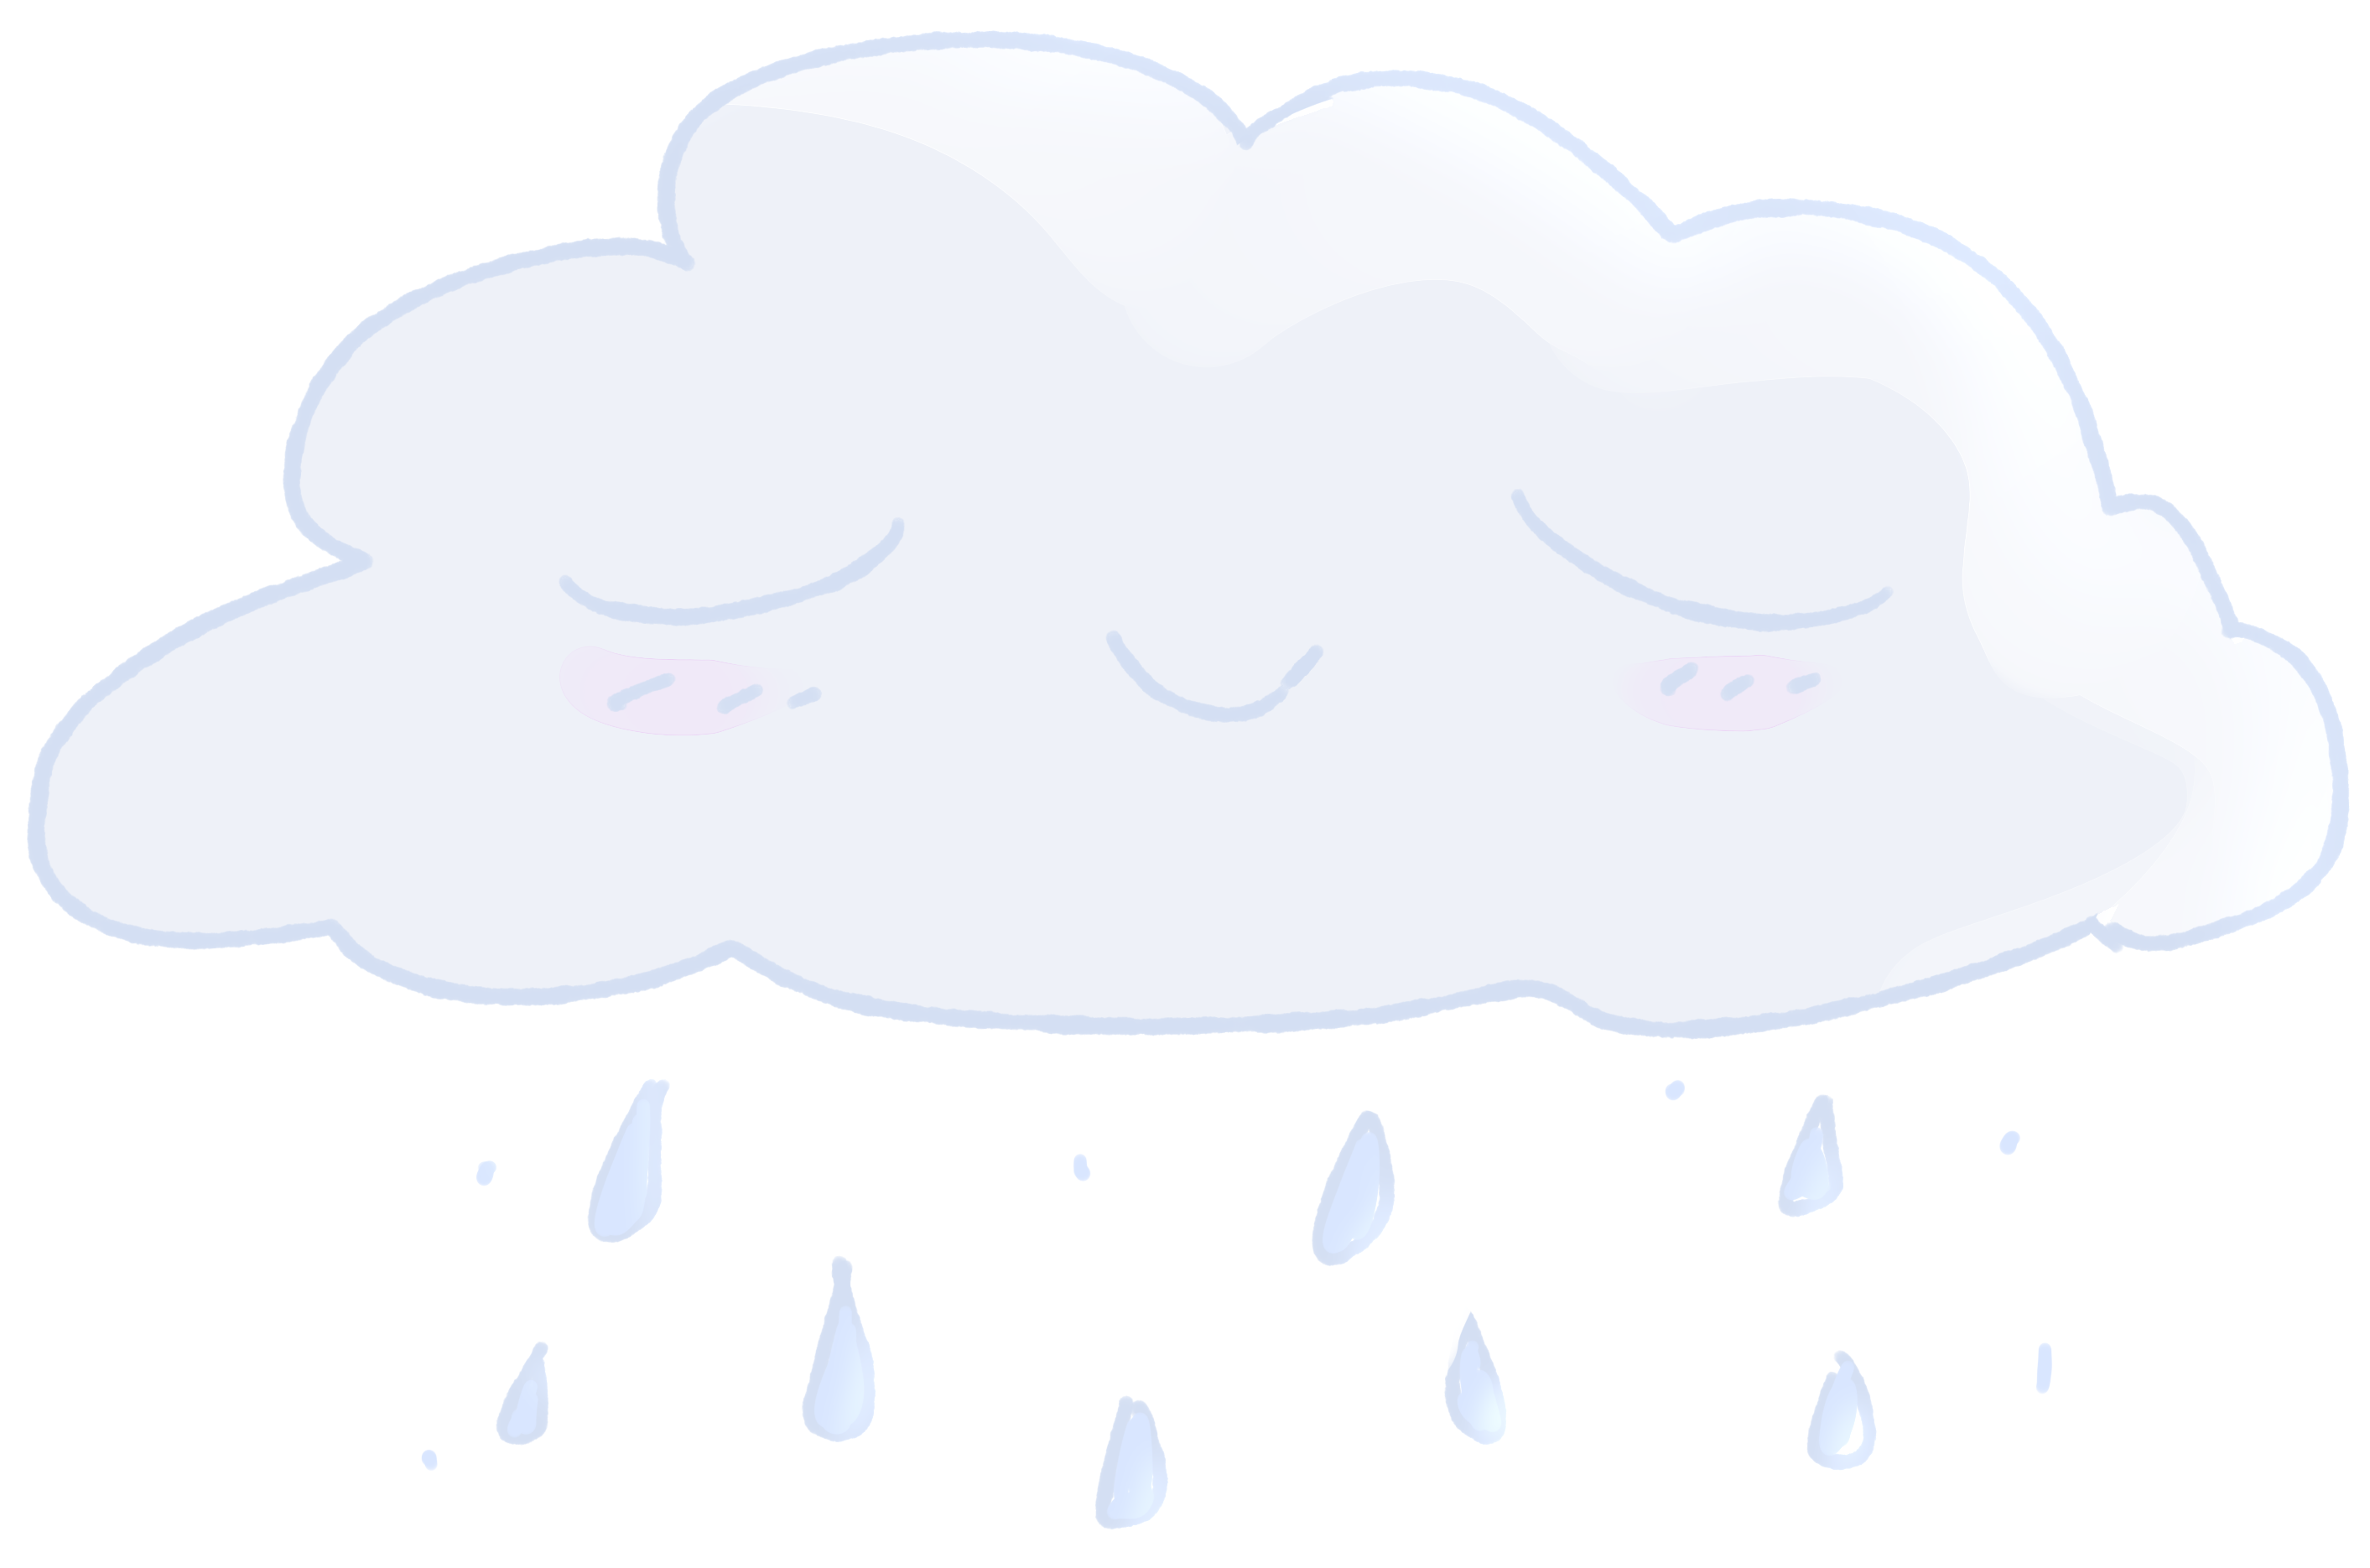
\includegraphics[scale=0.38]{resources/mrak2.png}}
\end{figure}
%%%%%%%%%%%%%%%%%%%%%%%%%%%%%%%%%%%%%%%%%%%%%%%%%%%%%%%%%%%%%%%%%%%%%%%%%%%%%%%%%%%%%%%%%%%%%%%%%%%%%%%%%%
\newpage
\section{Úlohy}
\begin{enumerate}

\item[a)] \textbf{Přiřaďte názvy k atmosférickým jevům.}
\newline 
(Skřítci, gigantická tryska, blesky, polární záře)
\begin{figure}[!thp]
\begin{minipage}[b]{0.4\textwidth}
    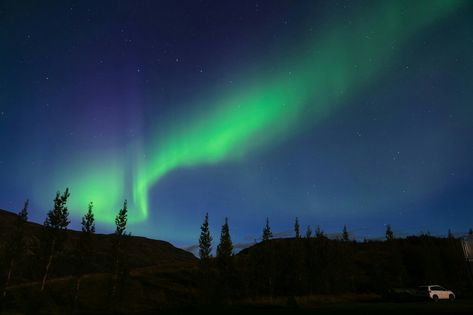
\includegraphics[width=\textwidth]{resources/aurora.jpg}
    
  \end{minipage}
  \hfill
  \begin{minipage}[b]{0.354\textwidth}
    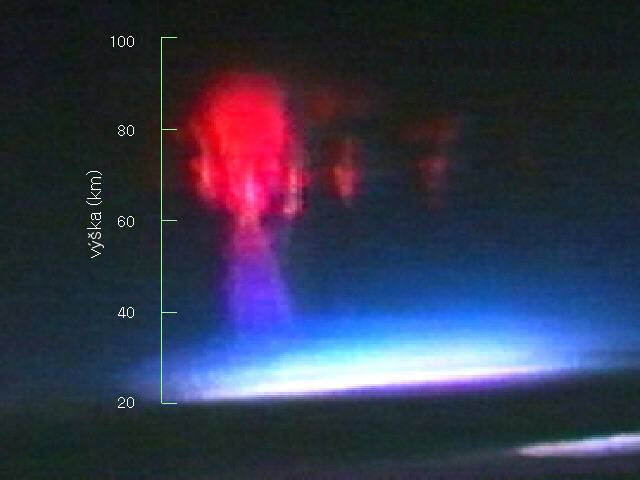
\includegraphics[width=\textwidth]{resources/skřítek.jpg}
    
  \end{minipage}
\end{figure}
\newline
\rule{4.5cm}{0.05cm} \hspace{5.7cm} \rule{3.5cm}{0.05cm}
\bigskip
\begin{figure}[tbh!]
\begin{minipage}[b]{0.5\textwidth}
    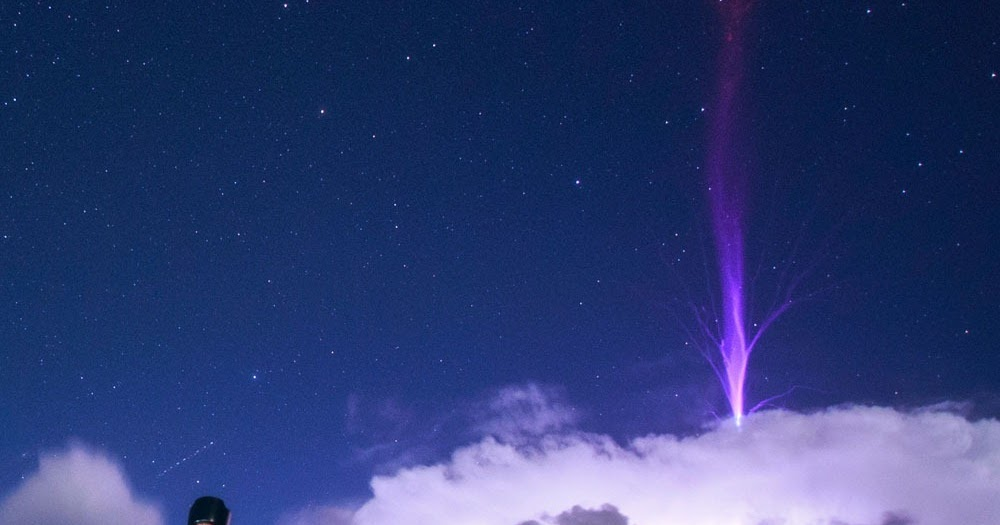
\includegraphics[width=\textwidth]{resources/jet.jpg}
    
  \end{minipage}
  \hfill
  \begin{minipage}[b]{0.272\textwidth}
    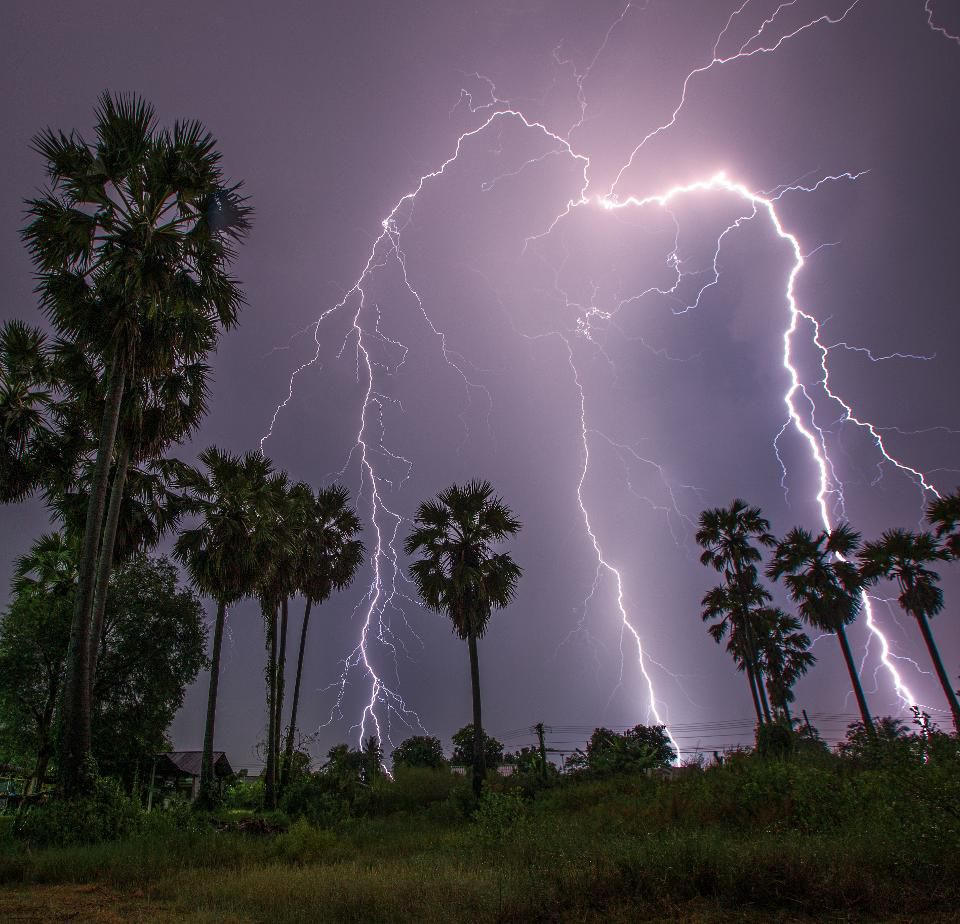
\includegraphics[width=\textwidth]{resources/blesk.jpg}
   
  \end{minipage}
   
\end{figure}


\rule{6cm}{0.05cm} \hspace{5cm} \rule{3.2cm}{0.05cm}

\item[b)]\textbf{Vyluštěte tajenku. Na některé otázky budete potřebovat použít i jiné zdroje.} 
\begin{small}


\begin{enumerate}
\item[1.] jev v termosféře, můžeme jej vidět na pólech, projevuje se jako zelená záře na obloze; latinsky 
\item[2.] výboje plazmy v mezosféře
\item[3.] silný výboj z mraku, doprovázen charakteristickým zvukem
\item[4.] perleťové zbarvení oblačnosti
\item[5.] můžeme tam pozorovat meteory
\item[6.] voda v atmosféře, ovlivňuje teplotu a vlhkost povrchu Země
\item[7.] astronaut, který čekal ve vesmíru na jeho kolegy při přistání Apolla 11
\item[8.] menší objekt vesmírného původu, který v atmosféře neshoří a doletí na zem

\end{enumerate}
\end{small}
\newpage
\begin{figure}[!tbh]
\begin{center}

    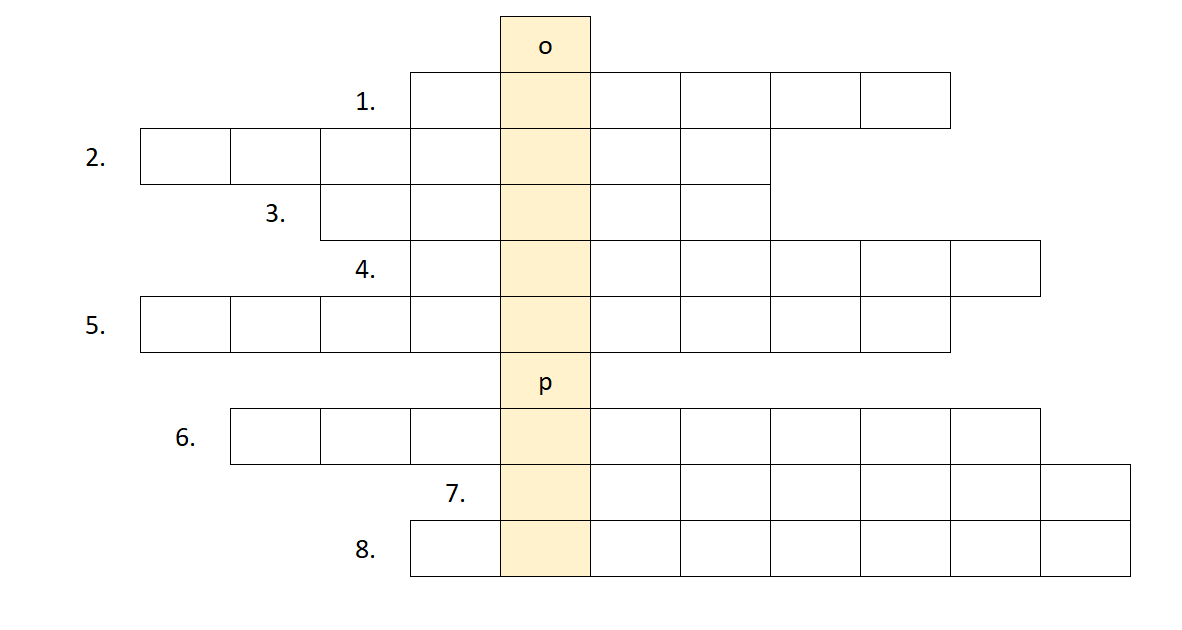
\includegraphics[scale=0.30]{resources/křížovka.png}
   
\end{center}
 {Řešení tajenky: }\rule{5cm}{0.05cm}
\end{figure}


 
\begin{multicols}{2}

\item[c)]\textbf{Spojte dvojice} 
\newline
\begin{center}



\begin{tabular}{|l|l|}
\hline
a) 78 \% atmosféry & 1.) voda   \\ \hline
b) 25-35 km       & 2.) kyslík \\ \hline
c) 0 - 10 km      & 3.) dusík  \\ \hline
d) 21 \% armosféry & 4.) ozon   \\ \hline
\end{tabular}
\end{center}
\begin{center}


\begin{tabular}{|l|l|l|l|}
\hline
a)\hspace{0.6cm} & b)\hspace{0.6cm} & c)\hspace{0.6cm} & d)\hspace{0.6cm} \\ \hline

\end{tabular}
\end{center}
\columnbreak
\item[d)]
\textbf{Napište alespoň 3 funkce\newline atmosféry.\newline Pomohou vám přesmyčky.}
\begin{enumerate}
\item chroaan řepd vu
\item lenpáte zaociel
\item dacnhíý	
\end{enumerate}
\end{multicols}
\item[e)]

\textbf{Má člověk vliv na atmosféru? Pozitivní nebo negativní? Jmenujte příklady.}

\bigskip
\bigskip
\bigskip

\item[f)] \textbf{BONUS: Zhlédněte video a odpovězte na otázky:}


\begin{minipage}{0.6\textwidth}
    
  \begin{enumerate}[label=(\Alph), itemsep=0pt]
  \item[1.] Co způsobuje polární záři?
  \bigskip
  \item[2.] Kde a proč právě tam ji můžeme pozorovat?
  \bigskip
  \item[3.] Do jaké velikosti se nafoukl jejich stratosférický\\ balon?
  \bigskip
  \item[4.] Kolik balonů vypustili a kolik z nich pořídilo fotky polární záře?
    \end{enumerate}
  
  \end{minipage}
  \begin{minipage}{0.3\textwidth}
   
\includegraphics[scale=0.14]{resources/qr.png}
   \url{https://www.youtube.com/watch?v=5O-wAYKBBSc}
  \end{minipage}
  

\end{enumerate}
\end{document}
